% Generated from Graphviz DOT by figures/make_figures.py; do not edit by hand.
\definecolor{slateink}{HTML}{334155}
\definecolor{slateedge}{HTML}{475569}
\definecolor{slatemid}{HTML}{64748B}
\definecolor{slatefill}{HTML}{F8FAFC}
\definecolor{orangefill}{HTML}{FFF7ED}
\definecolor{orangeedge}{HTML}{C2410C}
\definecolor{redfill}{HTML}{FEE2E2}
\definecolor{rededge}{HTML}{DC2626}
\definecolor{bluefill}{HTML}{DBEAFE}
\definecolor{blueedge}{HTML}{2563EB}
\definecolor{greenfill}{HTML}{DCFCE7}
\definecolor{greenedge}{HTML}{16A34A}
\definecolor{greenlight}{HTML}{F0FDF4}
\definecolor{greendark}{HTML}{15803D}
\definecolor{indigofill}{HTML}{EEF2FF}
\definecolor{indigoedge}{HTML}{4F46E5}
\definecolor{cyanfill}{HTML}{ECFEFF}
\definecolor{cyanedge}{HTML}{0891B2}
\definecolor{slatefillb}{HTML}{F1F5F9}
\definecolor{purplefill}{HTML}{FAE8FF}
\definecolor{purpleedge}{HTML}{A21CAF}
\definecolor{amberfill}{HTML}{FFFBEB}
\definecolor{amberedge}{HTML}{B45309}
\definecolor{pinkfill}{HTML}{FFF1F2}
\definecolor{bluelight}{HTML}{EFF6FF}
\definecolor{amberfillb}{HTML}{FEF3C7}
\definecolor{amberedgeb}{HTML}{D97706}
\definecolor{skyfill}{HTML}{E0F2FE}
\definecolor{skyedge}{HTML}{0284C7}
\definecolor{yellowfill}{HTML}{FEF9C3}
\definecolor{yellowedge}{HTML}{CA8A04}
\definecolor{orangefillb}{HTML}{FFEDD5}
\definecolor{orangeedgeb}{HTML}{EA580C}
\definecolor{grayfill}{HTML}{E2E8F0}
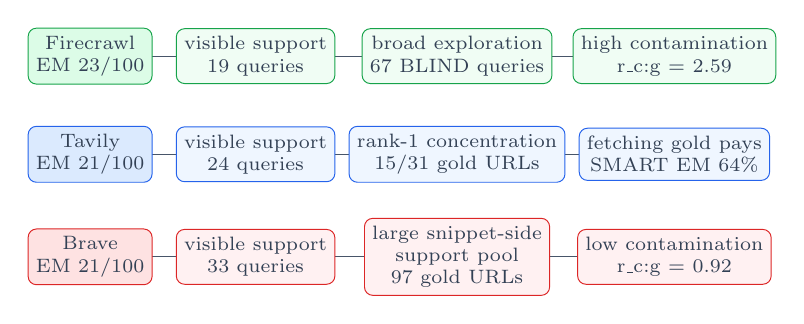
\begin{tikzpicture}[x=0.52in,y=0.52in,>=latex]
\tikzset{gvnode/.style={draw, rounded corners=3pt, align=center, font=\scriptsize, inner sep=2.8pt, line width=0.35pt}}
\tikzset{gvedge/.style={->, line width=0.35pt, color=slateedge}}
\draw[gvedge] (0.892,0.285) -- (0.892,0.285) -- (1.366,0.285) -- (1.366,0.285);
\draw[gvedge] (2.627,0.285) -- (2.627,0.285) -- (3.199,0.285) -- (3.199,0.285);
\draw[gvedge] (4.668,0.285) -- (4.668,0.285) -- (5.268,0.285) -- (5.268,0.285);
\draw[gvedge] (0.892,1.271) -- (0.892,1.271) -- (1.366,1.271) -- (1.366,1.271);
\draw[gvedge] (2.627,1.271) -- (2.627,1.271) -- (3.104,1.271) -- (3.104,1.271);
\draw[gvedge] (4.768,1.271) -- (4.768,1.271) -- (5.268,1.271) -- (5.268,1.271);
\draw[gvedge] (0.892,2.215) -- (0.892,2.215) -- (1.366,2.215) -- (1.366,2.215);
\draw[gvedge] (2.627,2.215) -- (2.627,2.215) -- (3.206,2.215) -- (3.206,2.215);
\draw[gvedge] (4.662,2.215) -- (4.662,2.215) -- (5.243,2.215) -- (5.243,2.215);
\node[gvnode, minimum width=0.462in, minimum height=0.260in, fill=redfill, draw=rededge, text=slateink] (b0) at (0.444,0.285) {Brave\\EM 21/100};
\node[gvnode, minimum width=0.614in, minimum height=0.260in, fill=pinkfill, draw=rededge, text=slateink] (b1) at (2.035,0.285) {visible support\\33 queries};
\node[gvnode, minimum width=0.722in, minimum height=0.296in, fill=pinkfill, draw=rededge, text=slateink] (b2) at (3.972,0.285) {large snippet-side\\support pool\\97 gold URLs};
\node[gvnode, minimum width=0.744in, minimum height=0.260in, fill=pinkfill, draw=rededge, text=slateink] (b3) at (6.062,0.285) {low contamination\\r\_c:g = 0.92};
\node[gvnode, minimum width=0.462in, minimum height=0.260in, fill=bluefill, draw=blueedge, text=slateink] (t0) at (0.444,1.271) {Tavily\\EM 21/100};
\node[gvnode, minimum width=0.614in, minimum height=0.260in, fill=bluelight, draw=blueedge, text=slateink] (t1) at (2.035,1.271) {visible support\\24 queries};
\node[gvnode, minimum width=0.823in, minimum height=0.260in, fill=bluelight, draw=blueedge, text=slateink] (t2) at (3.972,1.271) {rank-1 concentration\\15/31 gold URLs};
\node[gvnode, minimum width=0.744in, minimum height=0.260in, fill=bluelight, draw=blueedge, text=slateink] (t3) at (6.062,1.271) {fetching gold pays\\SMART EM 64\%};
\node[gvnode, minimum width=0.462in, minimum height=0.260in, fill=greenfill, draw=greenedge, text=slateink] (f0) at (0.444,2.215) {Firecrawl\\EM 23/100};
\node[gvnode, minimum width=0.614in, minimum height=0.260in, fill=greenlight, draw=greenedge, text=slateink] (f1) at (2.035,2.215) {visible support\\19 queries};
\node[gvnode, minimum width=0.715in, minimum height=0.260in, fill=greenlight, draw=greenedge, text=slateink] (f2) at (3.972,2.215) {broad exploration\\67 BLIND queries};
\node[gvnode, minimum width=0.773in, minimum height=0.260in, fill=greenlight, draw=greenedge, text=slateink] (f3) at (6.062,2.215) {high contamination\\r\_c:g = 2.59};
\end{tikzpicture}
